\documentclass[12pt,a4paper]{report}

\usepackage[utf8]{inputenc} % Codificação do arquivo
\usepackage[T1]{fontenc}    % Codificação da fonte
\usepackage[brazil]{babel}
\usepackage{graphicx,url}
\usepackage[top=2cm, bottom=2cm, left=2cm, right=2cm]{geometry}
\usepackage{hyperref}
\usepackage{cmap} % Mapear caracteres especiais no PDF
\usepackage{enumitem} % Para personalizar listas
\usepackage{amsmath} % Melhor suporte matemático
\usepackage{adjustbox} % Para ajustar o tamanho de imagens
\usepackage{float} % Para posicionar imagens

\hyphenpenalty=5000 % Evitar hifenização
\tolerance=1000     % Evitar ultrapassar margens

\begin{document}
	\begin{center}
		{\Large Universidade Federal de Uberlândia - UFU}
		
		Bacharelado em Sistemas de Informação
		
		\textbf{FACOM32504 - Redes de Computadores - 2024/2}
		
		\textbf{Arthur Fernandes - 11911BCC059}
	\end{center}
	
	\vspace{10pt}

	\begin{center}
		{\LARGE \textbf{Relatório 3 \\ \vspace{10pt} Domain Name System (DNS)}}
	\end{center}
	
	\vspace{10pt}
	
	\begin{figure}[ht]
		\centering
		
\includegraphics[width=0.3\textwidth]{ufu.png}
		\caption{Logo da UFU.}
		\label{fig:logoUFU1}
	\end{figure}

	\begin{enumerate}
		\item Execute o \texttt{nslookup} para obter o endereço IP de um servidor Web do Indian Institute of Technology em Bombaim, Índia: \texttt{www.iitb.ac.in}. Qual é o endereço IP desse servidor?
		
		\textbf{Resposta:} 

		\begin{figure}[H]
			\centering
			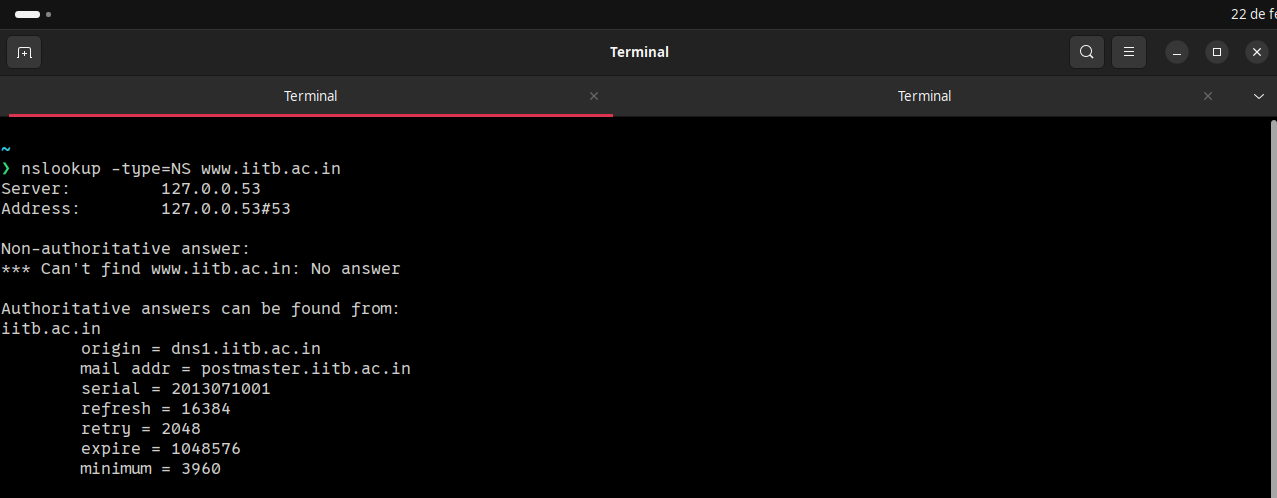
\includegraphics[width=1\textwidth]{q1.png}
			\caption{nslookup para o servidor www.iitb.ac.in (Questão 01)}
			\label{fig:q1}
		\end{figure}

		\item Qual é o endereço IP do servidor DNS que forneceu a resposta para o comando \texttt{nslookup} da questão 1?
		
		\textbf{Resposta:} O endereço IP do servidor DNS que forneceu a resposta, conforme mostrado na imagem 1 é 127.0.0.53.

		\item A resposta do comando \texttt{nslookup} da questão 1 foi obtida de um servidor DNS authoritative ou non-authoritative?
		
		\textbf{Resposta:} A resposta do comando \texttt{nslookup} da questão 1 foi obtida de um servidor DNS \textbf{non-authoritative}.

		\item Execute o comando \texttt{nslookup} para determinar os servidores DNS autorizados para uma universidade na Europa.
		
		\textbf{Resposta:}

		\begin{figure}[H]
			\centering
			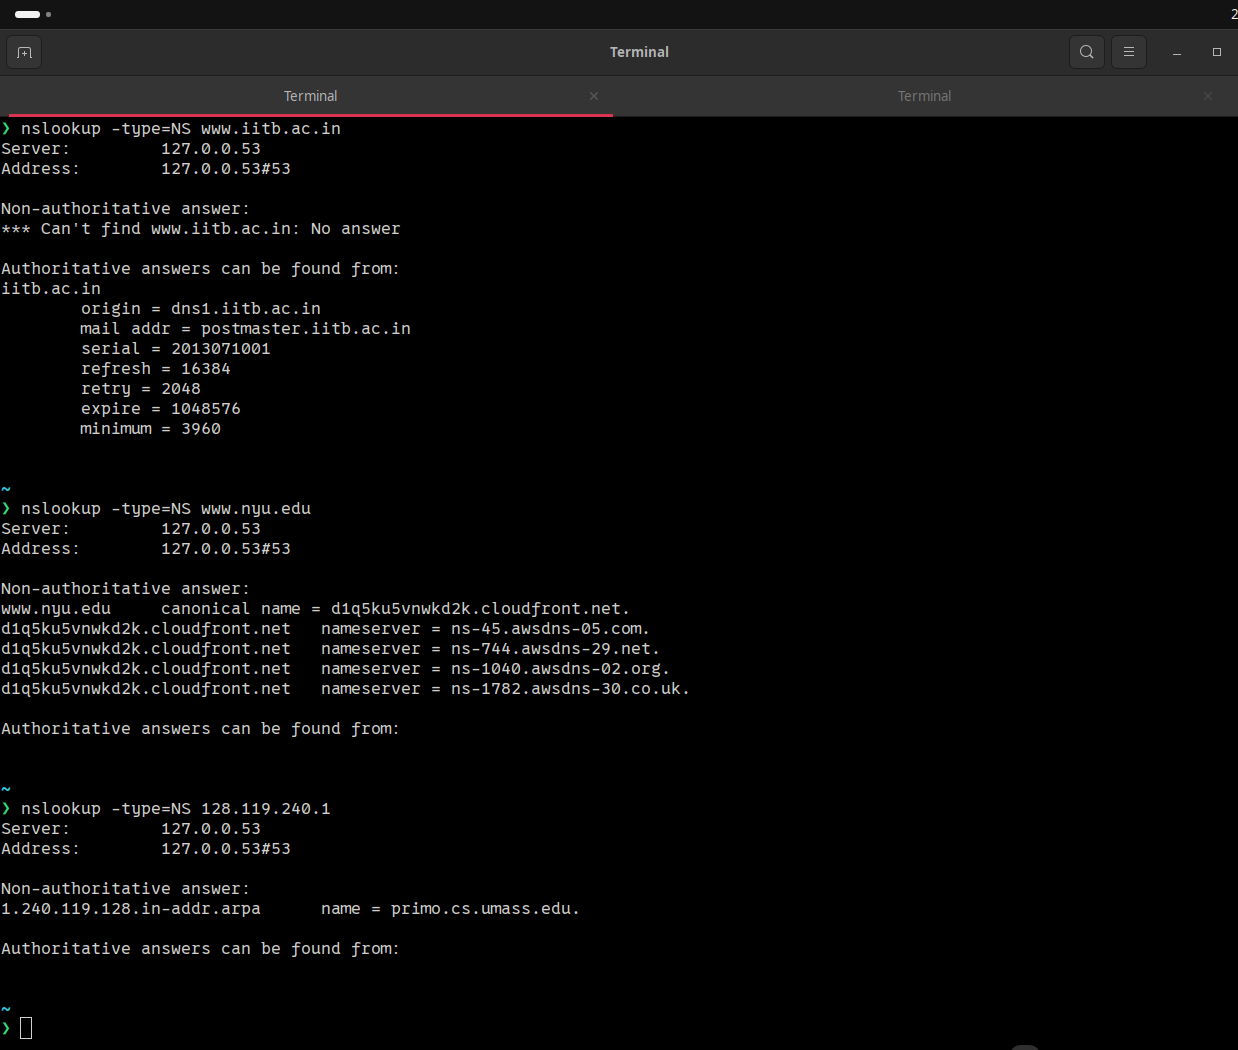
\includegraphics[width=1\textwidth]{q4.png}
			\caption{nslookup para determinar os servidores DNS autorizados (Questão 04)}
			\label{fig:q4}
		\end{figure}

		\item Localize a consulta DNS e as mensagens de resposta. Essas mensagens são enviadas via UDP ou TCP?
		
		\textbf{Resposta:} Via UDP.

		\begin{figure}[H]
			\centering
			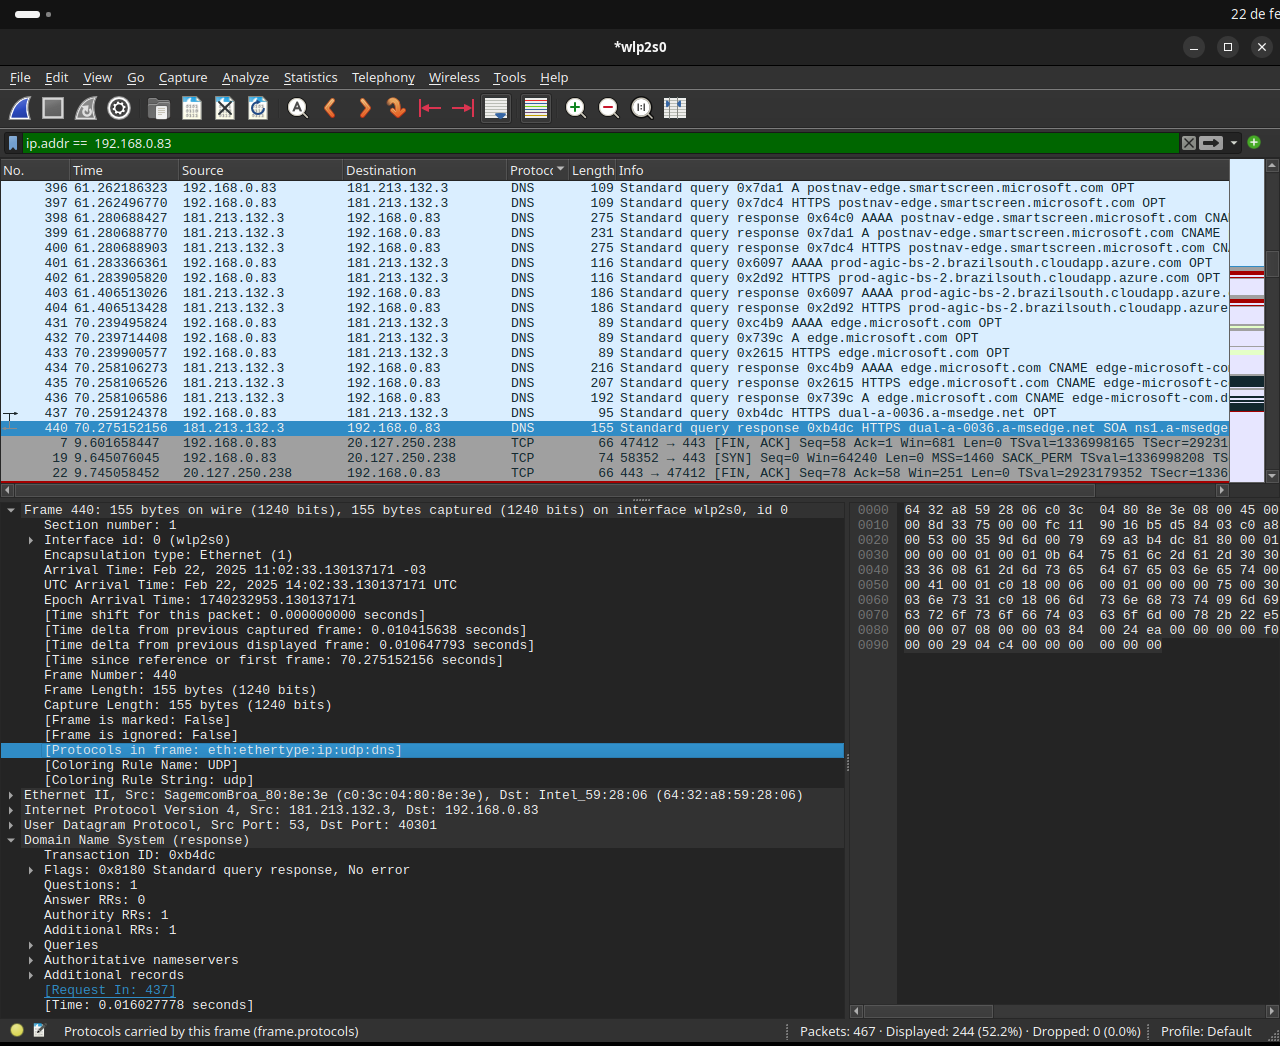
\includegraphics[width=1\textwidth]{q5.png}
			\caption{Como as mensagens foram enviadas (Questão 05)}
			\label{fig:q5}
		\end{figure}

		\item Qual é a porta de destino da mensagem de consulta DNS? E qual é a porta de origem da mensagem de resposta DNS?
		
		\textbf{Resposta:} Souce Port: 40301 e Destination Port: 53. Agora em Standard Query Response, Source Port: 53 e Destination Port: 40301.

		\item Para qual endereço IP é enviada a mensagem de consulta DNS? Utilize o comando \texttt{ipconfig} para verificar o endereço IP do seu servidor DNS local. Esses dois endereços IP são iguais?
		
		\textbf{Resposta:} 

		\begin{figure}[H]
			\centering
			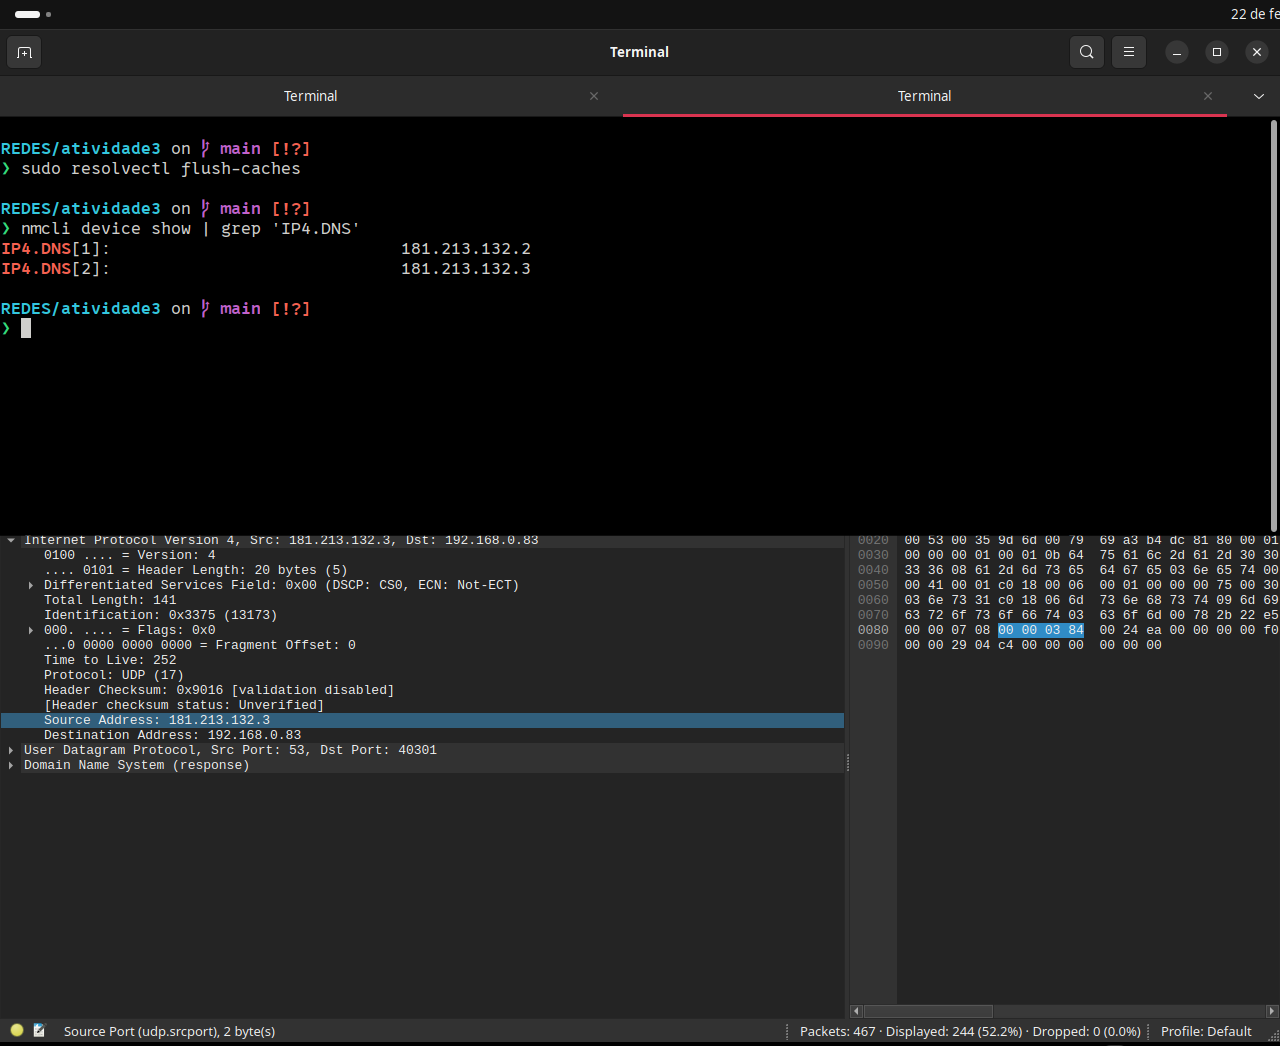
\includegraphics[width=1\textwidth]{q7.png}
			\caption{Endereço IP do servidor DNS local (Questão 07)}
			\label{fig:q7}
		\end{figure}

		\item Analise a mensagem de consulta DNS: qual é o “tipo” de consulta realizada? A mensagem de consulta contém alguma “resposta”?
		
		\textbf{Resposta:}

		\begin{figure}[H]
			\centering
			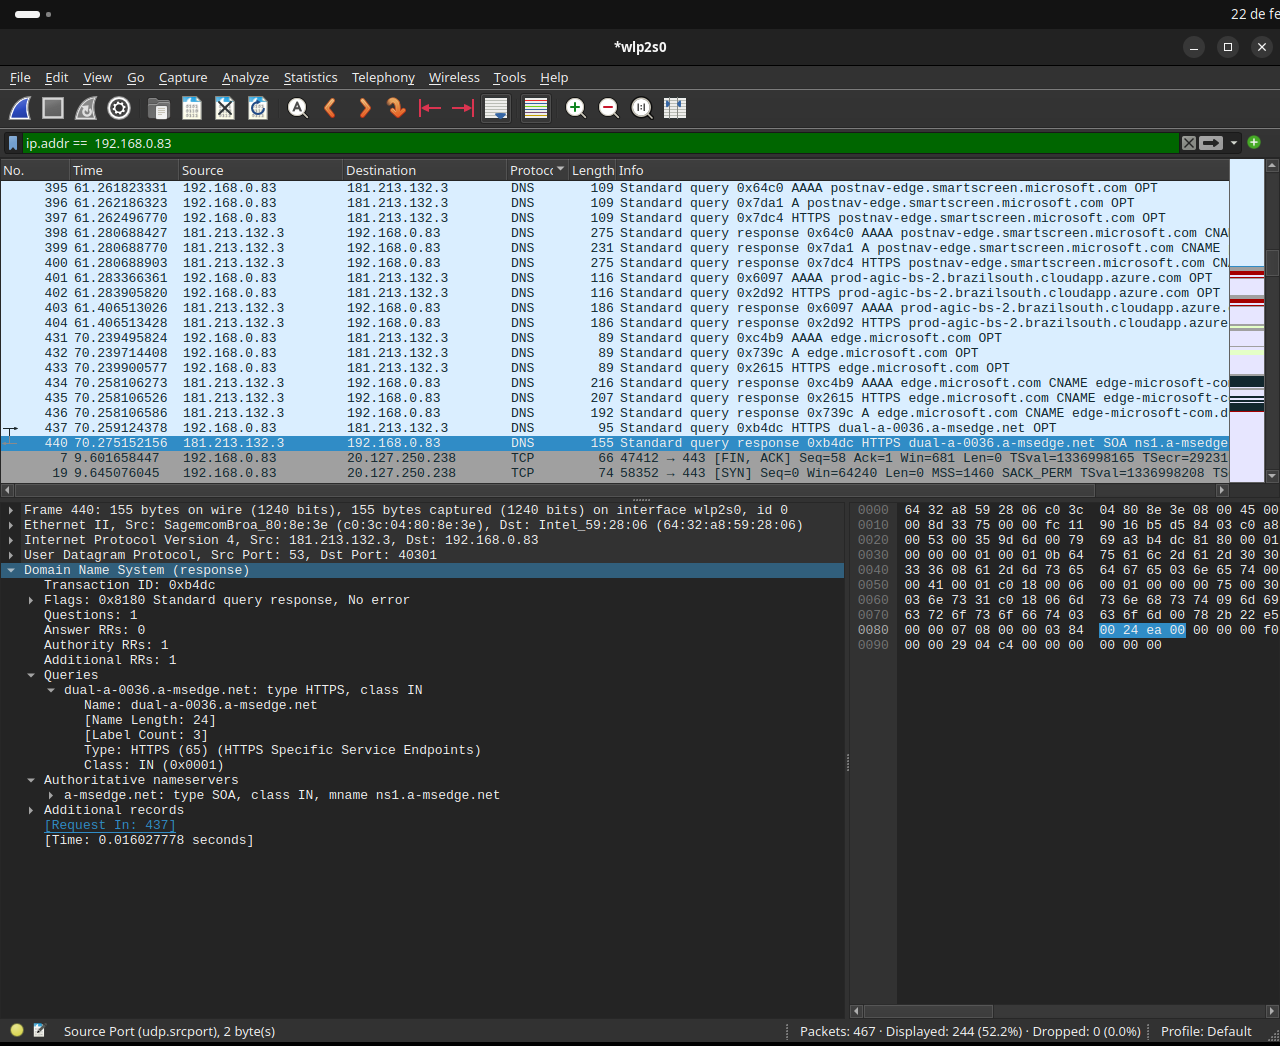
\includegraphics[width=1\textwidth]{q8.png}
			\caption{Tipo de consulta realizada (Questão 08)}
			\label{fig:q8}
		\end{figure}

		\item Analise a mensagem de resposta DNS: quantas “respostas” são fornecidas e o que cada uma delas contém?
		
		\textbf{Resposta:} Nenhuma resposta.

		\item Considere o pacote TCP SYN subsequente enviado pelo seu host. O endereço IP de destino desse pacote corresponde a algum dos endereços IP apresentados na mensagem de resposta DNS?
		
		\textbf{Resposta:} Não consegui entender muito bem essa.

		\item A página base disponível em \url{http://gaia.cs.umass.edu/kurose_ross/} faz referência à imagem \url{http://gaia.cs.umass.edu/kurose_ross/header_graphic_book_8E_2.jpg}, sendo ambas hospedadas em \texttt{gaia.cs.umass.edu}.
		
		\begin{enumerate}
			\item Qual é o número do pacote no rastreamento da solicitação HTTP GET inicial para o arquivo base?
			
			\textbf{Resposta:}

			\begin{figure}[H]
				\centering
				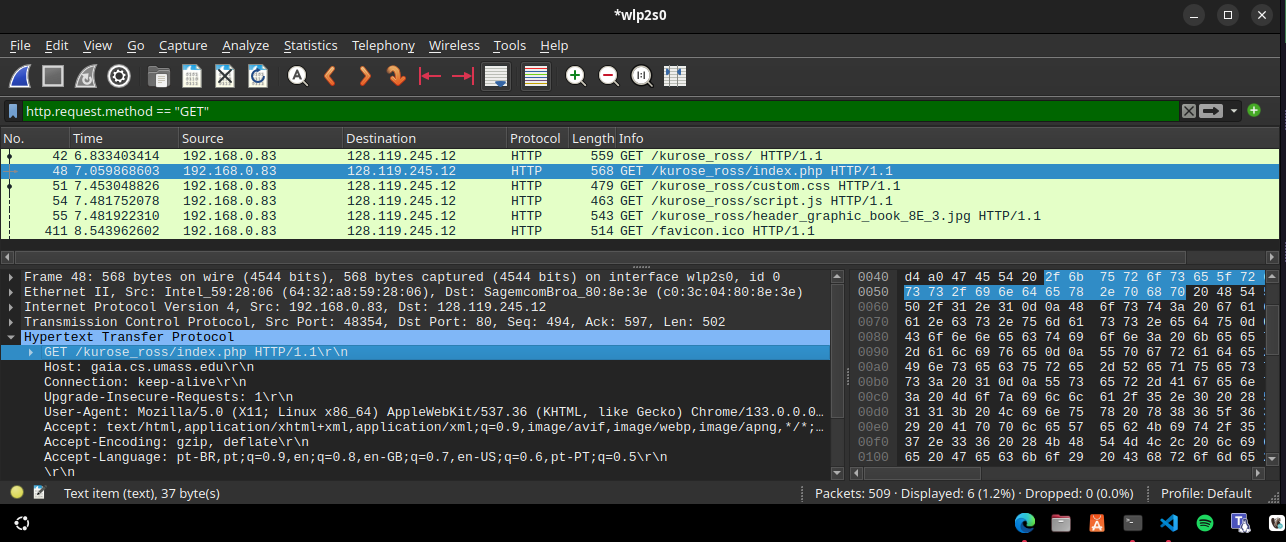
\includegraphics[width=1\textwidth]{q11a.png}
				\caption{Número do pacote no rastreamento da solicitação HHTP GET inicial (Questão 11 a)}
				\label{fig:11a}
			\end{figure}

			\item Qual é o número do pacote no rastreamento da consulta DNS realizada para resolver gaia.cs.umass.edu, permitindo o envio da solicitação HTTP inicial para o endereço IP correspondente?
			
			\textbf{Resposta:} O número do pacote é 11. Conforme mostra a figura 11b.

			\begin{figure}[H]
				\centering
				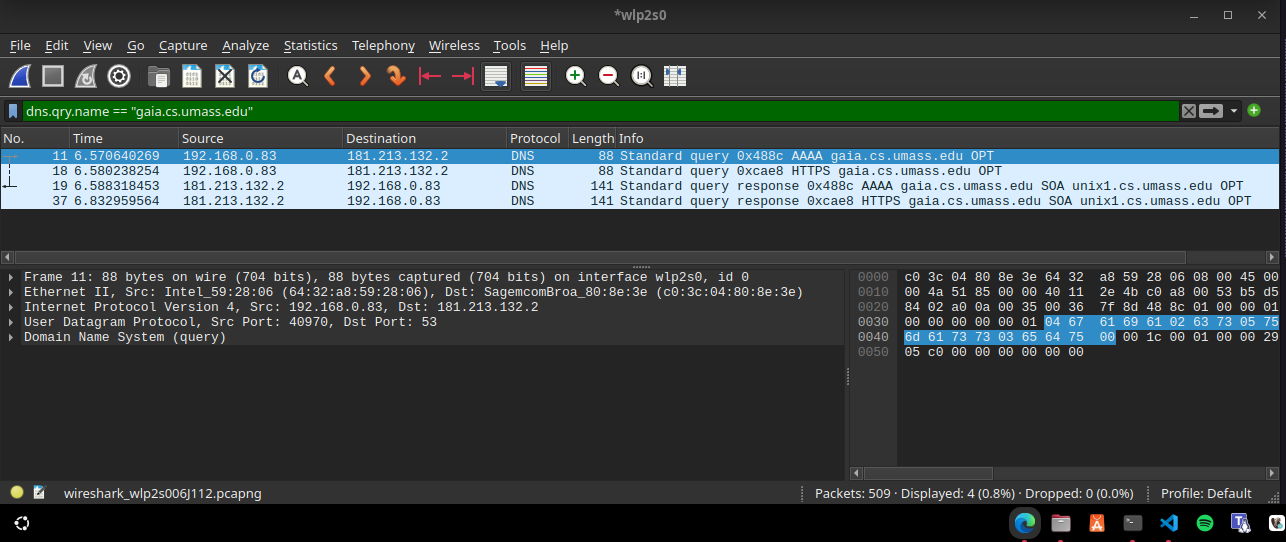
\includegraphics[width=1\textwidth]{q11b.png}
				\caption{Número do pacote no rastreamento da consulta DNS (Questão 11 b)}
				\label{fig:11b}
			\end{figure}

			\item Qual é o número do pacote no rastreamento da resposta DNS recebida?
			
			\textbf{Resposta:} Está no pacote 19 conforme mostra a figura 11b.

			\item Qual é o número do pacote no rastreamento da solicitação HTTP GET para o objeto de imagem?
			
			\textbf{Resposta:} pacote de numero 55 conforme a imagem abaixo.

			\begin{figure}[H]
				\centering
				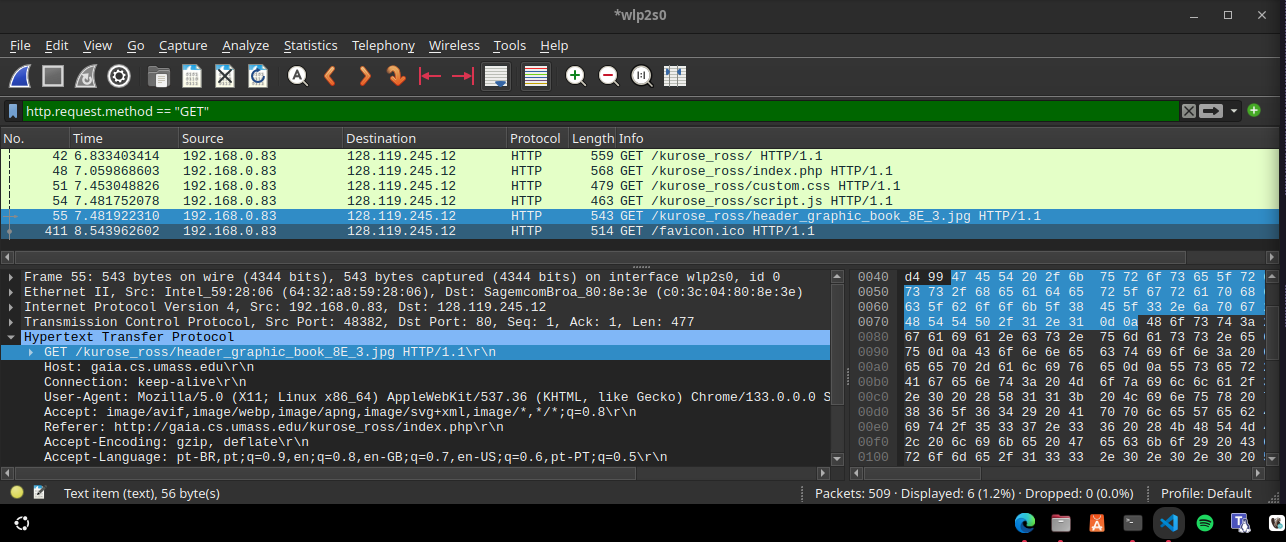
\includegraphics[width=1\textwidth]{q11d.png}
				\caption{Número do pacote no rastreamento da solicitação HTTP GET para o objeto de imagem (Questão 11 d)}
				\label{fig:11d}
			\end{figure}

			\item Qual é o número do pacote referente à consulta DNS efetuada para para resolver \url{gaia.cs.umass.edu}
			para que esta segunda solicitação HTTP possa ser enviada para o endereço IP gaia.cs.umass.edu?
			
			\textbf{Resposta:} pacote de numero 18 conforme a imagem abaixo.

			\begin{figure}[H]
				\centering
				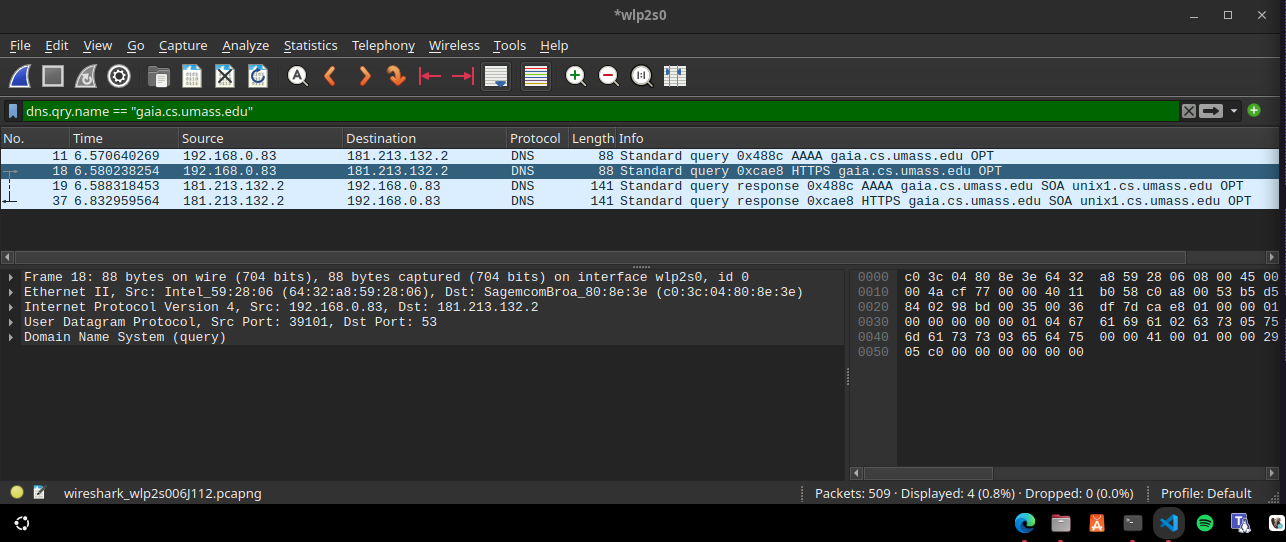
\includegraphics[width=1\textwidth]{q11e.png}
				\caption{Número do pacote referente à consulta DNS (Questão 11 e)}
				\label{fig:11e}
			\end{figure}
		\end{enumerate}

		\item Qual é a porta de destino para a mensagem de consulta DNS? E qual é a porta de origem da mensagem de resposta DNS?
		
		\textbf{Resposta:} porta de destino 53 e porta de origem 53. Conforme mostra a imagem abaixo, usando a porta 19 como exemplo.

		\begin{figure}[H]
			\centering
			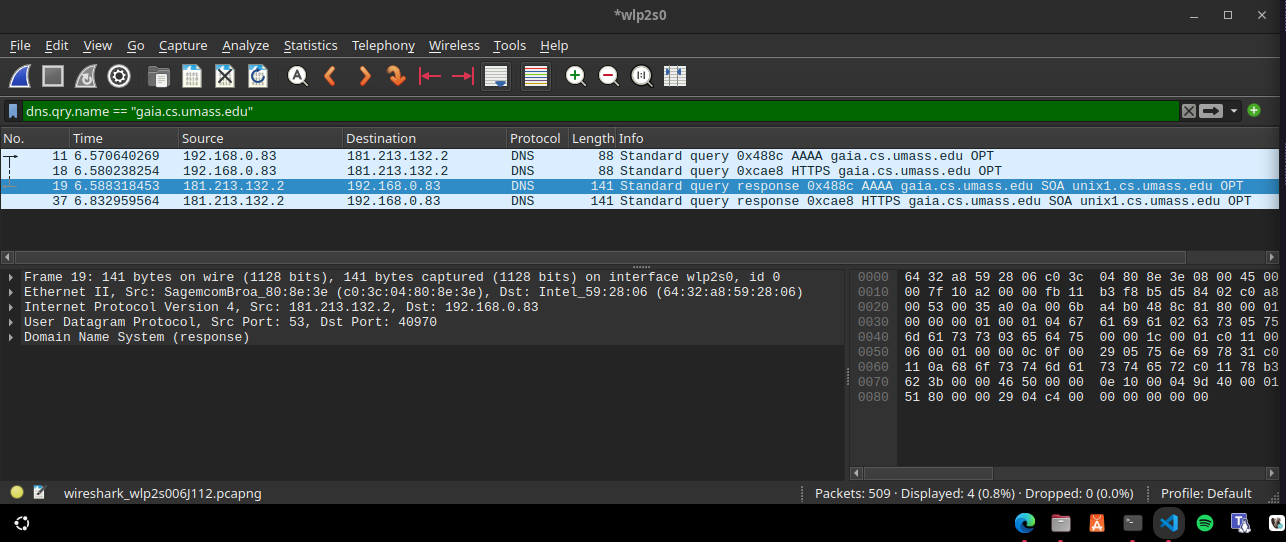
\includegraphics[width=1\textwidth]{q12.png}
			\caption{Portas de destino e origem (Questão 12)}
			\label{fig:12}
		\end{figure}

		\item Para qual endereço IP é enviada a mensagem de consulta DNS? Esse endereço IP corresponde ao do seu servidor DNS local padrão?
		
		\textbf{Resposta:} a consulta DNS foi enviada para o endereço IP 181.213.132.2. Sim, corresponde ao endereço IP do servidor DNS local padrão, veja na imagem abaixo.

		\begin{figure}[H]
			\centering
			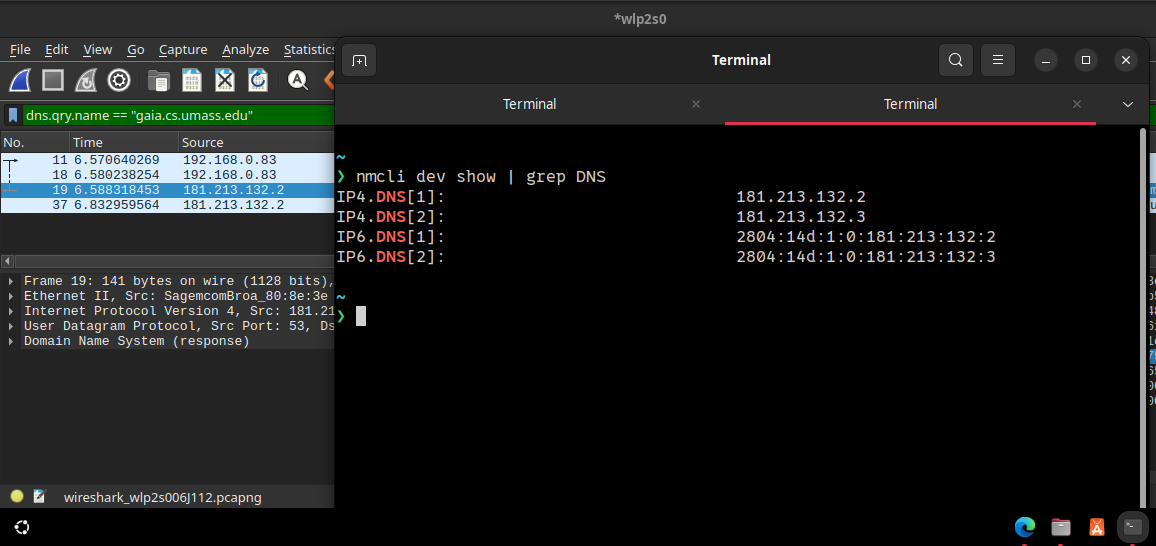
\includegraphics[width=1\textwidth]{q13.png}
			\caption{Endereço IP do servidor DNS local padrão (Questão 13)}
			\label{fig:13}
		\end{figure}

		\item Analise a mensagem de consulta DNS: qual é o “tipo” de consulta efetuada? A mensagem de consulta contém alguma “resposta”?
		
		\textbf{Resposta:} Foi o tipo de query AAAA. Não contém resposta.

		\item Analise a mensagem de resposta DNS: quantas “respostas” são fornecidas e o que cada uma delas contém?
		
		\textbf{Resposta:} Contém duas respostas, pacotes 19 e 37. Contém uma resposta para o pacote 11 e outra para o pacote 18, respectivamente.

		\begin{figure}[H]
			\centering
			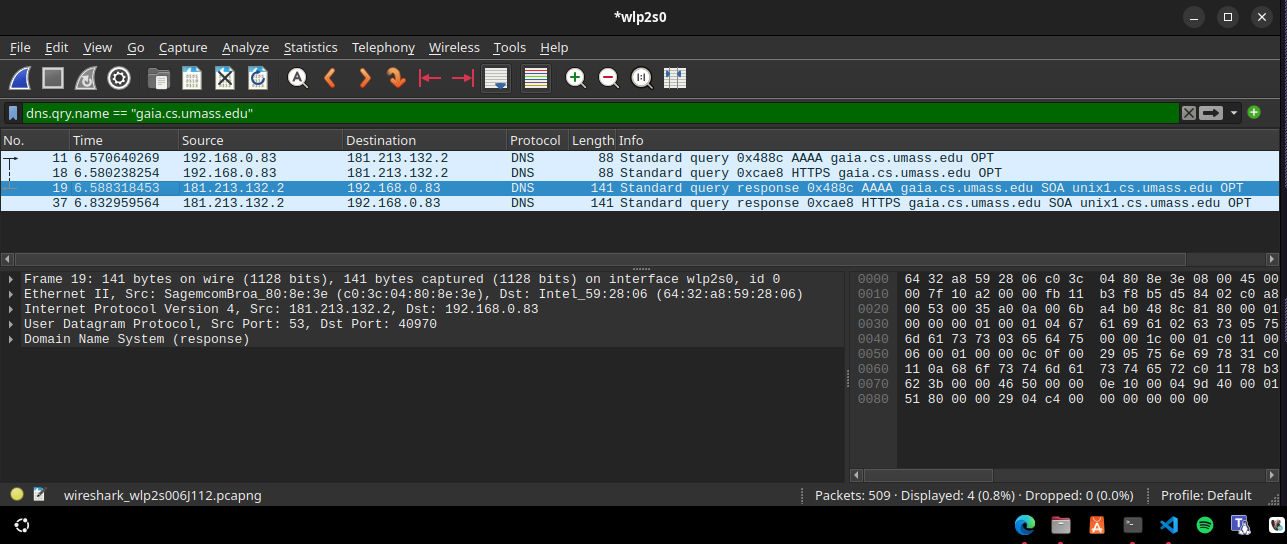
\includegraphics[width=1\textwidth]{q15.png}
			\caption{Respostas fornecidas (Questão 15)}
			\label{fig:15}
		\end{figure}

		\item Para qual endereço IP é enviada a mensagem de consulta DNS? Esse endereço IP corresponde ao do seu servidor DNS local padrão?
		
		\textbf{Resposta:} Já foi respondido na questão 13.

		\item Analise novamente a mensagem de consulta DNS: qual é o “tipo” de consulta efetuada? A mensagem de consulta contém alguma “resposta”?
		
		\textbf{Resposta:} Já foi respondido na questão 14.

		\item Analise a mensagem de resposta do DNS:
		
		\begin{enumerate}
			\item Quantas respostas estão presentes?
			
			\textbf{Resposta:} Duas respostas, conforme o print da questão 15.

			\item Quais informações estão contidas em cada uma dessas respostas?
			
			\textbf{Resposta:} Resposta está na questão 15.

			\item Quantos registros de recursos adicionais foram retornados?
			
			\textbf{Resposta:} Os dois prints abaixo motram os registros adicionais retornados.

			\begin{figure}[H]
				\centering
				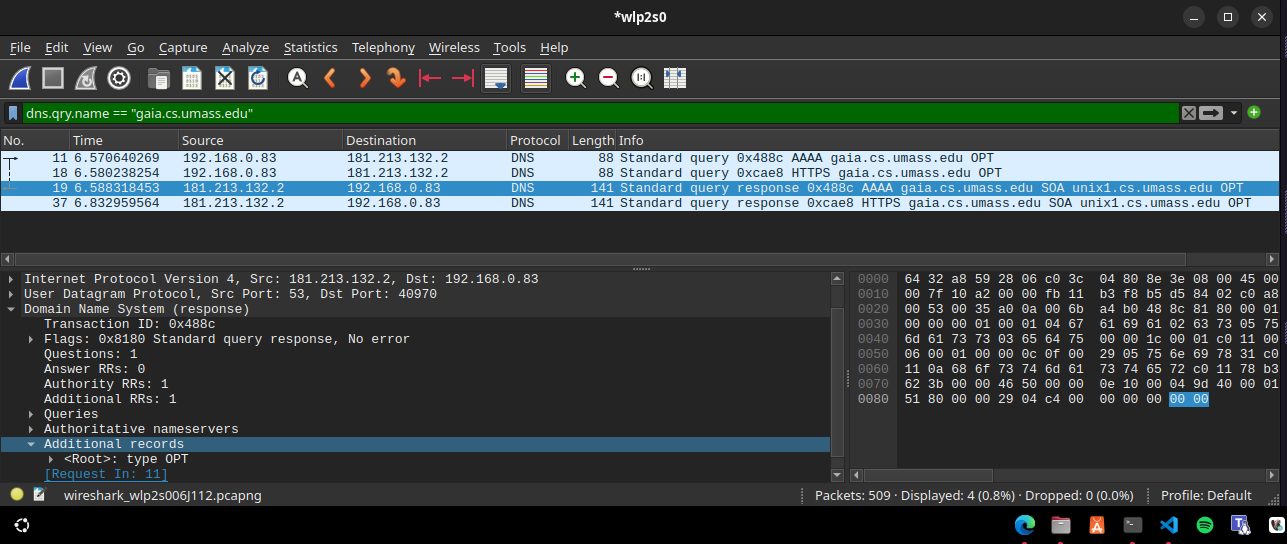
\includegraphics[width=1\textwidth]{q18c.png}
				\caption{Registros adicionais retornados (Questão 18 c)}
				\label{fig:18c}
			\end{figure}

			\begin{figure}[H]
				\centering
				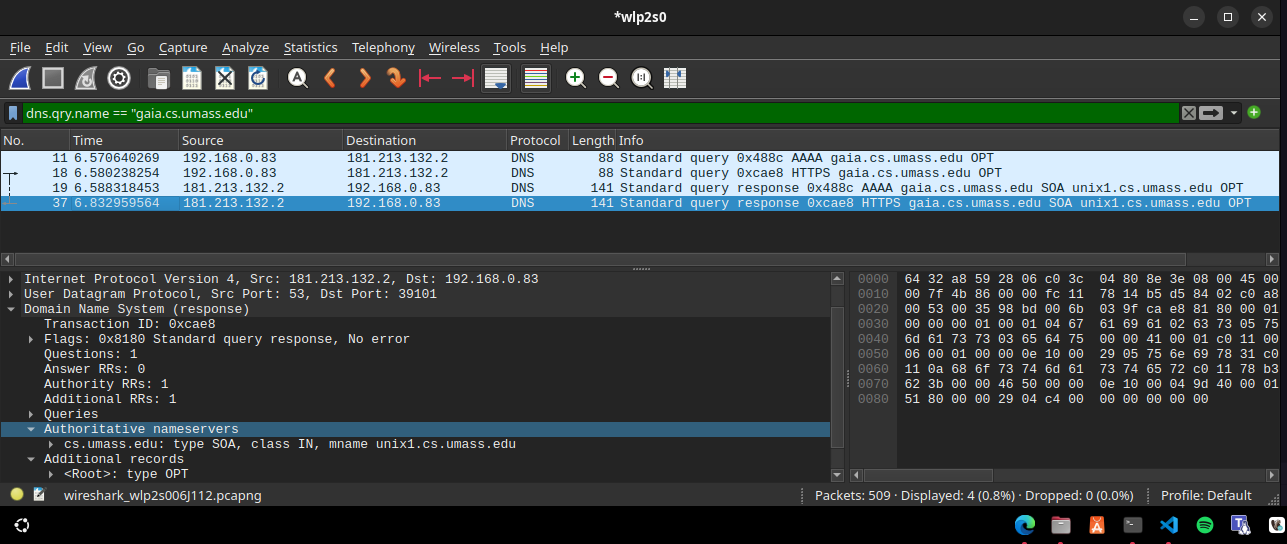
\includegraphics[width=1\textwidth]{q18c2.png}
				\caption{Registros adicionais retornados (Questão 18 c)}
				\label{fig:18c2}
			\end{figure}

			\item Quais informações adicionais estão incluídas nesses registros?
			
			\textbf{Resposta:} <Root>: type OPT.
		\end{enumerate}

		\item Para qual endereço IP é enviada a mensagem de consulta DNS? Esse é o endereço IP do seu servidor DNS local padrão? Caso contrário, a que endereço IP ele corresponde?
		
		\textbf{Resposta:}  Respondido na questão 13. Caso contrário eu não entendi muito bem.

		\item Analise a mensagem de consulta DNS: qual é o “tipo” de consulta efetuada? A mensagem de consulta contém alguma “resposta”?
		
		\textbf{Resposta:}Respondido na questão 14.

		\item Analise a mensagem de resposta DNS: quantas “respostas” são fornecidas e o que cada uma delas contém?
		
		\textbf{Resposta:} Questão 18 responde aqui também.
		
	\end{enumerate} 

\end{document}
